\section{Результаты}

Программа получает на вход два параметра: количество экспериментов (\texttt{--rounds N}) и максимальное число потоков (\texttt{--max-threads M}). После проверки корректности аргументов она запускает многопоточное моделирование методом Монте-Карло: каждый поток независимо выполняет заданное число раундов, в каждом из которых создаётся и перемешивается колода из 52 карт, после чего проверяется, совпадают ли достоинства двух верхних карт.\\
По завершении всех вычислений программа выводит в стандартный поток вывода:
\begin{itemize}
    \item общее число проведённых раундов,
    \item количество успешных исходов (совпадение достоинств),
    \item экспериментальную вероятность в виде десятичной дроби,
    \item время выполнения как в наносекундах, так и в секундах.
\end{itemize}
Результатом работы является численная оценка вероятности, которая при увеличении числа раундов стремится к теоретическому значению $\frac{3}{51} \approx 0.0588 (5.88\%)$.\\
Программа корректно обрабатывает ошибочные ситуации (некорректные аргументы, недопустимые значения) и завершается с кодом ошибки. В случае корректного запуска все потоки завершаются штатно, ресурсы освобождаются автоматически, а результат выводится без искажений. Реализация на основе \texttt{std::thread} обеспечивает кроссплатформенность и безопасную параллельную обработку данных.\\
График зависимости времени от количества используемых потоков приведен \\на рисунке 1.(\texttt{rounds = $10^7$}).
Анализ показывает, что при увеличении числа потоков от 1 до 12 наблюдается устойчивое сокращение времени выполнения, что свидетельствует о хорошей параллелизуемости задачи. Ускорение достигает примерно 6.3× (21.10 / 3.34) при использовании 12 потоков по сравнению с однопоточной версией.\\
Минимальное время выполнения достигается при 12 потоках, после чего дальнейшее увеличение числа потоков не приводит к ускорению, а, напротив, вызывает незначительный рост времени. Это объясняется тем, что количество рабочих потоков превышает число логических ядер процессора, доступных в системе. В результате операционная система вынуждена выполнять переключение контекста между потоками, что порождает дополнительные накладные расходы на управление потоками, конкуренцию за кэш процессора и снижение общей эффективности выполнения.\\
Таким образом, оптимальное число потоков для данной задачи и аппаратной конфигурации составляет 12, что, соответствует количеству логических ядер центрального процессора. Полученные результаты подтверждают общее правило: для CPU-ограниченных задач максимальная производительность достигается при числе потоков, равном числу логических ядер системы. Дальнейшее увеличение параллелизма нецелесообразно и может привести к деградации производительности.
\begin{figure}[h]
    \centering
    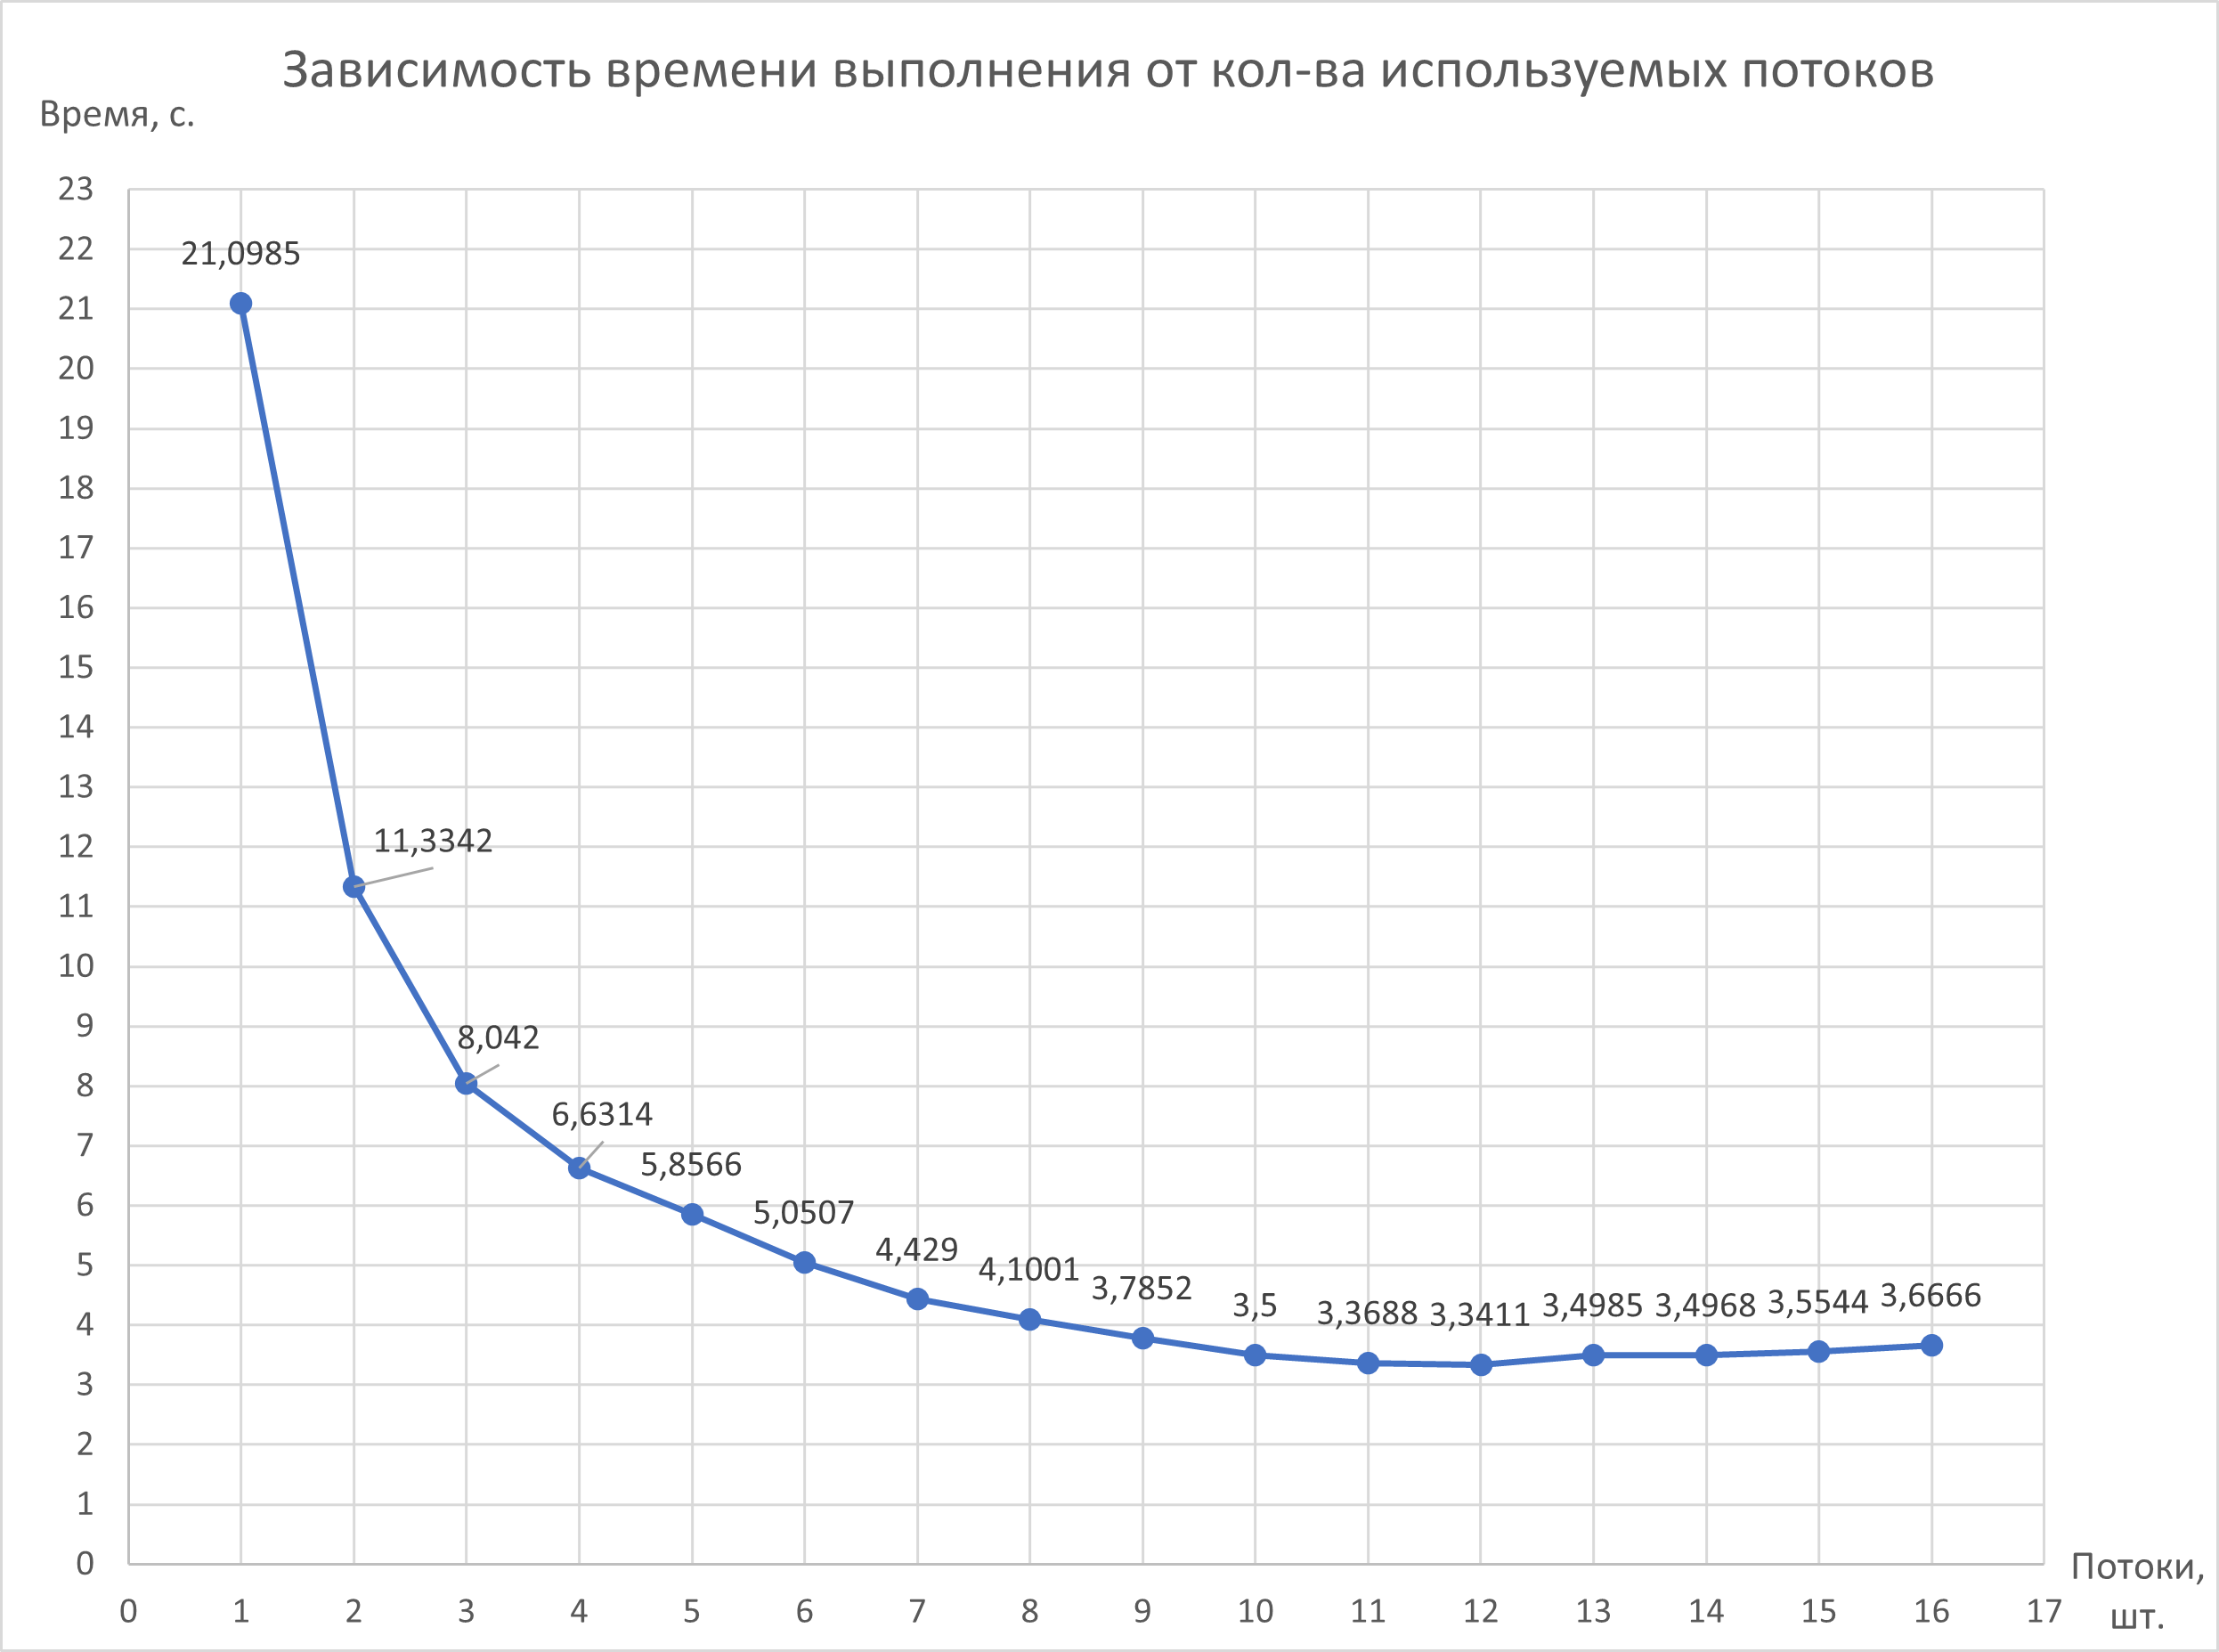
\includegraphics[width=0.75\textwidth]{src/graph.png}
    \caption{График зависимости времени выполнения от количества используемых потоков.}
    \label{fig:graph}
\end{figure}